\chapter{Outcomes of the IO-SEA project}

The different outcomes are directly related to the different work packages of the project. This is why they are
exposed WP after WP.

As a reminder, the technical Work Packages are
\begin{itemize}
    \item \textbf{Work Package \#1~:} \textit{Use Case and Co-design~:} this WP primarily characterizes the use
    cases and provides a detailed understanding of the requirements which is then used to develop an initial
    blueprint of the IO-SEA system, including all the components of the infrastructure. The work package also
    works on the adaptation of these use cases to fit to the IO-SEA architecture.
    
    \item \textbf{Work Package \#2~:} \textit{Data Workflow and Ephemeral~:} this WP focuses on providing an
    on-demand data access environment suitable for the needs of applications and workflows within the IO-SEA
    project. The on-demand data access environment will be Ephemeral – that is, it will be provisioned and
    available only during the runtime of the workflow. At the end of the workflow, the data access environment is
    torn down and any data and state are flushed to the backend storage tiers.
    
    \item \textbf{Work Package \#3~:} \textit{Instrumentation and Monitoring~:} this WP focuses on collecting and
    analysing Applications and Workflows IO behaviour, as well as IO infrastructure health. The information will
    be used to take optimum dimensioning and placement decisions when launching new instances of workflows.
    
    \item \textbf{Work Package \#4~:} \textit{Hierarchical Storage Management Feature~:} this WP aims is to
    provide Hierarchical Storage Management (HSM) for the IO-SEA architecture, making it capable of managing
    storage “NVMe to Tapes” tiers including various types of devices (NVRAM, Flash, SSD, HDD and Tapes). This is
    achieved by using together two object stores: the Mero Object store from Seagate and Phobos, a tape-based open
    source object store developed by CEA. 
    
    \item \textbf{Work Package \#5~:} \textit{Application Interfaces~:} this WP focuses on the interfaces exposed
    by the data placement and storage system. Requirements identified in WP1 will help shaping the API that will
    be offered to applications. This API will enable applications to interact with the system, describing data
    flow as managed by WP2 and storage policies used by WP4. The use-cases described in WP1 will be adapted to 
    use the API.
\end{itemize}

\section{Outcomes from WP1}

\section{Outcomes from WP2}

The main outcomes from the second work package are related to the creation of the workflow manager. Since
ephemeral service are strongly associated to compute jobs, the following schema is to be respected
\begin{enumerate}
    \item allocate the compute nodes to run the simulation jobs
    \item allocate the data nodes in order to run the ephemeral services
    \item start the ephemeral services
    \item make the ephemeral services accessible to the compute nodes, for example mounting a NFS share
    exposed via a NFS ephemeral service
    \item run the simulation
    \item if several steps are involved in the simulation, run the other steps of the simulation
    \item end the simulation
    \item flush the data to the persistent storage (typically the object stores)
    \item stop the ephemeral services
    \item release the data nodes and the compute nodes
\end{enumerate}

The WP2 made all the development to achieve this schema. The main outcome developed in the Workflow manager,
which makes it possible to manage the allocation of temporary IO servers, or ephemeral servers, implemented in 
the IO-SEA. As compute jobs are running on compute nodes, ephemeral services are working on data nodes, which
are part of dedicated modules within the MSA (see \ref{fig:msa}). 

The Workflow Manager operates as described in figure \ref{fig:wfm}. The concept of compute job is replaced by
the more complete concept of workflow. A workflow is made of different steps, where simulation program are run
as well as ephemeral service. 

\begin{figure}[H]
    \centering
    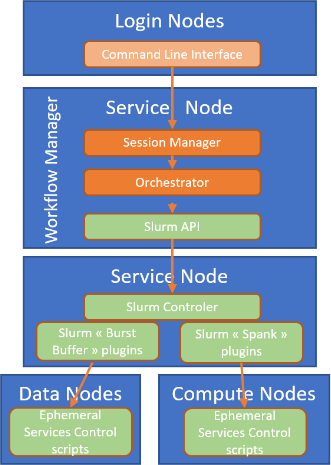
\includegraphics[width=0.35\textwidth]{FIGS/wfm.png}
    \caption[Worflow Manager Architecture]{ Worflow Manager Architecture}
    \label{fig:wfm}
\end{figure}

The workflow contains explicit dependencies, for example you need to have an
already started ephemeral IO server before you can do actual IO operations. The workflow is described by a 
workflow description file, written in JSON. 

The Workflow Manager is a key component inside the IO-SEA, it's a central place where all pieces are set
together. The user requirements from WP1 drove most of the development of this feature and operated in clode
collaboration with WP2. The WFM starts and uses the ephemeral servers developed by WP4 as well as elaborated
user interfaces provided by WP5. 

Inside the Workflow Manager resides an orchestrator whose tasks is to allocate and start all the executables
involved in a workflow. From this perspective, the orchestrator has strong acquaintance with the compute center's
resource scheduler (such as Slurm). The figure \ref{fig:it4i} showns how such a framework was deployed on the 
OpenStack Cloud hosted at IT4I, it is an actual proof that the workflow manager actually works. 

\begin{figure}[H]
    \centering
    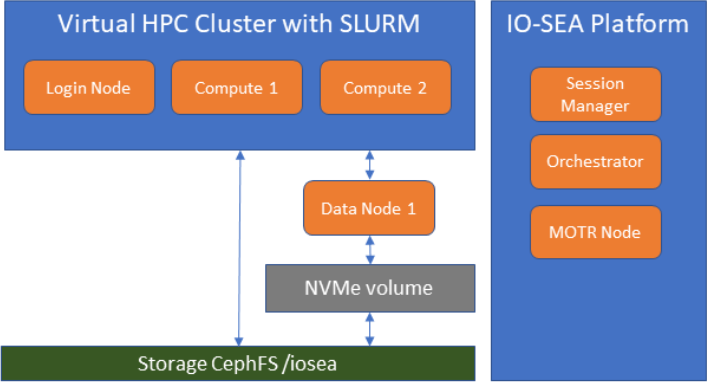
\includegraphics[width=0.75\textwidth]{FIGS/it4i.png}
    \caption[Worflow Manager at IT4I]{Instances deployed at IT4I OpenStack Cloud}
    \label{fig:it4i}
\end{figure}

The Workflow manager comes with itw own API and a set of command-line utility that help in efficiently manage
the workflow related operations (such a "start" / "stop" or "pause" / "resume"). 


\section{Outcomes from WP3}

The third Work Package of the IO-SEA project makes a focus on instrumentation and monitoring, plus the
development of tools to extract useful bits of information from the collected data. 

During the three years run of IO-SEA, WP3 has succeeded in developing a fine instrumentation framework able to
get hardware and software probes. In particular, the WP3 utility makes it possible to observe and measure the 
behavior of applications. By having a fine understanding of the mechanisms involved in the different core
components of IO-SEA, mostly used in WP2 and WP4. This makes it possible to put probes at the exact right 
location, exposing quite relevant data.

\begin{figure}[H]
    \centering
    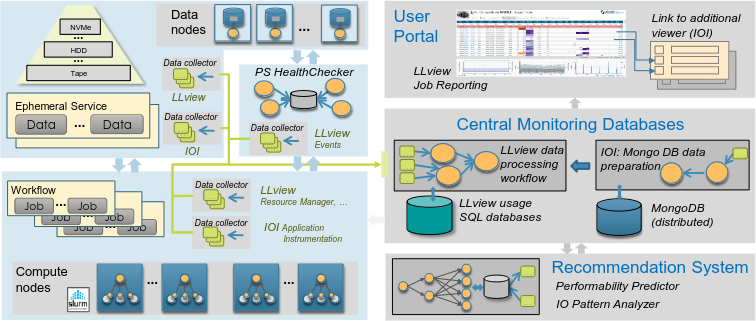
\includegraphics[width=0.75\textwidth]{FIGS/io_instr.png}
    \caption[I/O Monitoring architecture]{ The Architecture of the I/O monitoring framework}
    \label{fig:instr}
\end{figure}

This data is collected in databases, and can be later displayed via interactive 
GUI. Such integration as for example been done in tools via LLView or ParaStation HealthChecker. Giving a clear
overview is interesting, but this is not the only benefit of WP3, the instrumentation databases are dug via 
AI framework in order to build a \textit{recommendation system}. This new feature helps in identifying patterns
in the user application, opening the path to optimising those applications. Within the scope of the IO-SEA
project, such a recommendation systems could automatically add "hints" on objects or datasets, helping WP4 and
the HSM feature capable of using this hints as an input in their internal policies.

\begin{figure}[H]
    \centering
    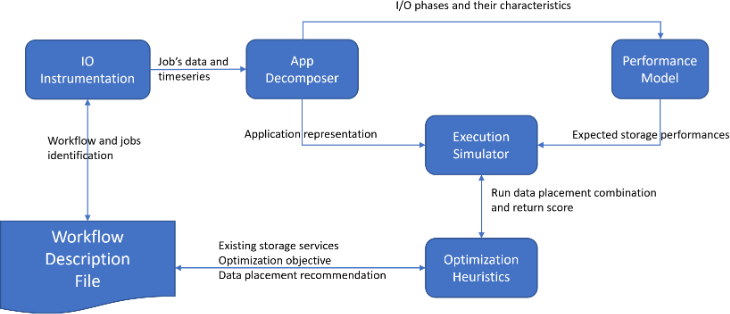
\includegraphics[width=0.75\textwidth]{FIGS/recom.png}
    \caption[Recommendation system]{ The general architecture of the recommendation system}
    \label{fig:recom}
\end{figure}

A side effect of this work is the "IO Traces Collection" initiative supported by both projects, ADMIRE and
IO-SEA. This initiative offers a non intrusive instrumentation framework whose well formatted output should be
stored in a common database, hosted on the internet and available to everyone. Researchers could use this tool
to work on optimisation for they have a large zoo of many different application behaviors. 





\section{Outcomes from WP4}

Several outcomes come from the WP4. During the three years of the project, it became obvious that a clear 
management of a generic HSM made it necessary to have a defined API and a defined architecture. This API, name HESTIA (ADD MEANING OF THE ACRONYM), make this possible. HESTIA is not attached to any feature of a given object 
store. In IO-SEA, it brings all the tools needed to implement the HSM feature between Phobos and another object
store.

The HESTIA API models and formalises ways to use various storage technologies  like NVMe, SSD, HDD, or tape, to
allow object stores to handle every type of device within the same storage hierarchy. It will make IO-SEA 
capable of dealing with the complete lifecycle of the data inside the same system. This system will be capable of managing most of the existing storage devices, from NVMe to tapes. To achieve this, it leverages two open-source
object stores: CORTX-Motr on top of Phobos (with the necessary abstractions to support additional backends).
Thus, HSM mechanisms are implemented in two products, making them capable of managing data movements between
them. The figure \ref{fig:hestia} depicts how the different compoments are organised within the HESTIA 
framework. 

\begin{figure}[H]
    \centering
    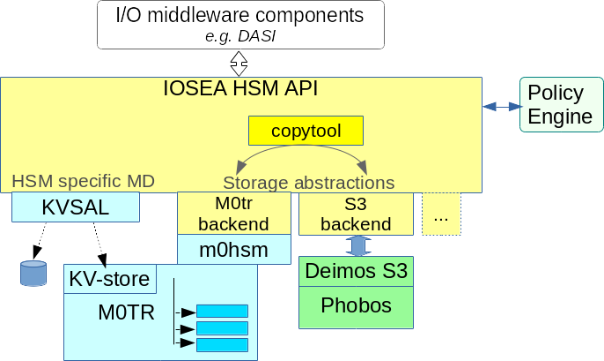
\includegraphics[width=0.75\textwidth]{FIGS/hestia.png}
    \caption[HESTIA software architecture]{ The architecture of the HESTIA framework}
    \label{fig:hestia}
\end{figure}

Hestia is an open source project that can be found at \url{https://git.ichec.ie/io-sea-internal/}.

HESTIA manages the data movement and triggers some of them internally (e.g. for managing data migration as data
have become cold enough to be migrated to tapes). The Robinhood software (available at
\url{https://github.com/cea-hpc/robinhood}, is the policy engine used to achieve that goal. 

PHOBOS, or \textit{Parallel Heterogeneous OBject Store}, is an object store developed at CEA and available as an
open-source software at \url{https://github.com/cea-hpc/phobos}. PHOBOS existed before the beginning of IO-SEA,
but was strongly improved during the three years of the project. PHOBOS is designed to manage large volumes of
data for various kinds of storage technologies from SSD to tapes. Phobos can efficiently handle very large
datasets on inexpensive media without sacrificing scalability, performance, or fault-tolerance requirements.

Phobos is designed to allow the easy integration of new modules for layouts such as mirroring and erasure coding
or I/O adapters. It's architecture can be seen on figure \ref{fig:phobos}. 

\begin{figure}[H]
    \centering
    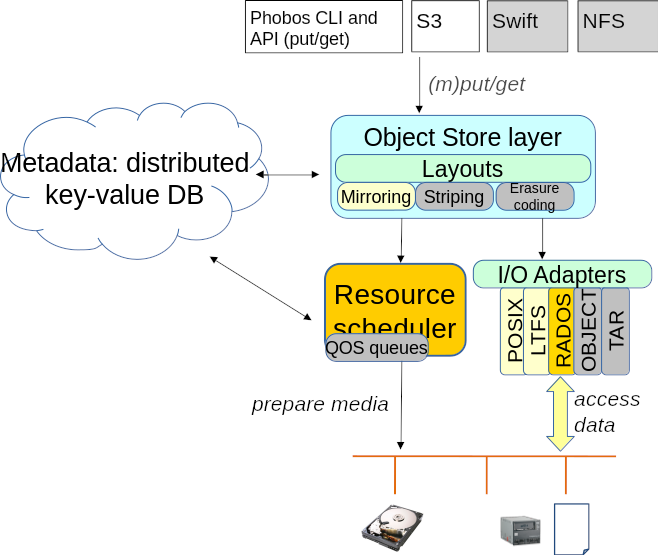
\includegraphics[width=0.75\textwidth]{FIGS/phobos.png}
    \caption[PHOBOS architecture]{ The architecture of the PHOBOS software}
    \label{fig:phobos}
\end{figure}

KVSNS is a library that makes it possible to implement a POSIX semantic on top of the services provided by an
object store and a key-value store. KVSNS was originally developed in the run of the SAGE and SAGE2 project, but
the related version was not capable of managing object store with only a CRUD\footnote{Create Read Update Delete}
interface, the object store had to be capable of performing random I/O operations in objects, just like POSIX
does via the \verb|pread()| or \verb|pwrite()| from the LibC. Inside IO-SEA, KVSNS gain a new feature, making it
capable of dealing with CRUD-only obbject store. This required the introduction of a local filesystem used as
a cache and a way to fetch and dispose entry from/to this cache. This logic should not be a bottleneck, it should
be implemented as a fully parallel and distributed service. This lead to the development of the GRH feature.
It's layers are described by figure \ref{fig:kvsns}

\begin{figure}[H]
    \centering
    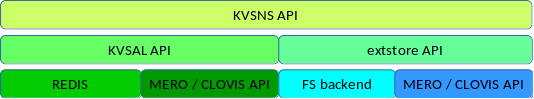
\includegraphics[width=0.75\textwidth]{FIGS/KVSNS_architecture.png}
    \caption[KVSNS layers]{ The layers of the KVSNS library}
    \label{fig:kvsns}
\end{figure}

GRH gets request issued by the KVSNS library itself, or externally. It creates an asynchronous request id that
can be used by the client to get the status of the request in an asynchronous way. GRH implement workers and 
tasks queues. GRH is based on the Celery framework, which is strongly parallel. GRH could be used outside its
original scope.In particular, GRH can be used to implement a data mover. The overall architecture of the GRH is
described by figure \ref{fig:grh}. 

\begin{figure}[H]
    \centering
    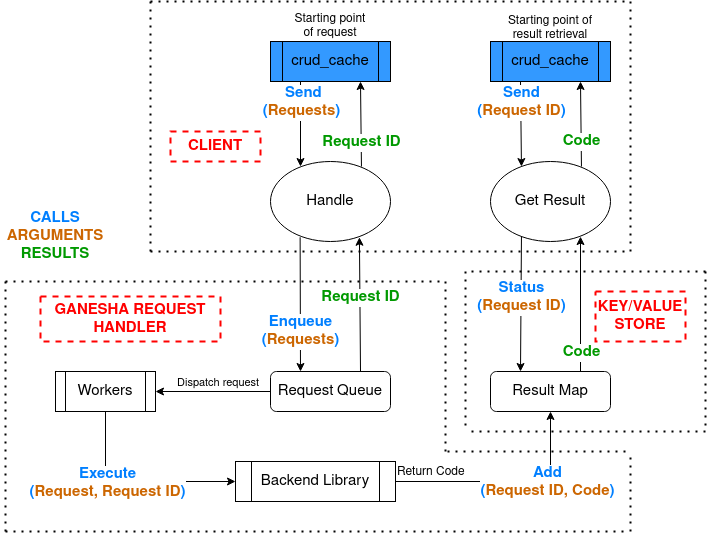
\includegraphics[width=\textwidth]{FIGS/GRH.png}
    \caption[GRH architecture]{ The design of the GRH component}
    \label{fig:grh}
\end{figure}

IO-SEA strongly relies on object stores. Implementing the IO-SEA architecture from scratch is easy, as new
data will be inserted inside directly in the object store, but what about moving data, already stored in standard
distributed and parallel file-systems? It's important to implement the required tools to make it possible to 
migrate data from the previously existing storage systems. One of the promises in the IO-SEA's proposal is 
providing such a framework. This goal was actually achieved as shown in figure \ref{fig:migration-path}. 

\begin{figure}[H]
    \centering
    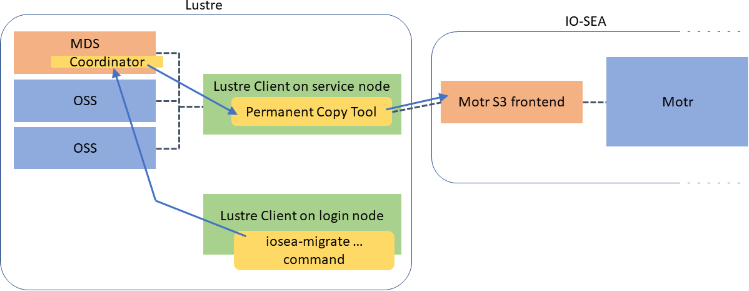
\includegraphics[width=0.75\textwidth]{FIGS/migration-path.png}
    \caption[Migration Path]{ The migration path in the IO-SEA}
    \label{fig:migration-path}
\end{figure}

\section{Outcomes from WP5}

The main outcome of the WP5 is the \textit{Data Access Storage Interface}, or \textbf{DASI}. 
DASI (available at \url{https://github.com/io-sea/dasi}) is a semantic interface for data, where the data is
indexed and uniquely identified by sets of scientifically-meaningful metadata keys. DASI is modular and is
compatible with multiple backends (i.e., object stores or POSIX) through diverse frontends (Python, C++, C).

Internally, DASI is based on software developed by ECMWF, named FDB2, which has been developed in previous EU
projects (NEXTGenIO), but has been heavily adapted and extended to be agnostic of and configurable for
different scientific domains. Leveraging FDB in this way means that many backends are already supported by DASI,
including a high-performance POSIX backend, a Ceph object storage backend, and an NVRAM backend. During the
IO-SEA project, a backend will also be created for CORTX. Applications will have seamless access to these
backends once they have been modified to support DASI. The DASI architecture is shown in figure \ref{fig:dasi}
as well as its dependency to other work done in the scope of IO-SEA.

\begin{figure}[H]
    \centering
    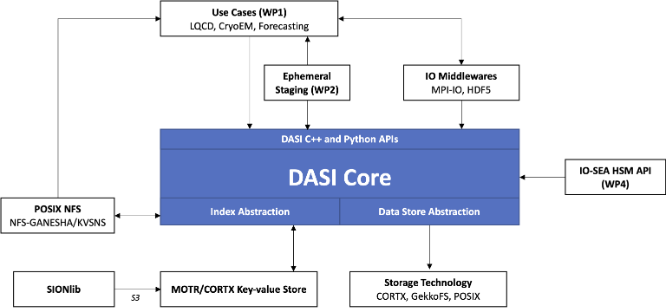
\includegraphics[width=0.75\textwidth]{FIGS/dasi.png}
    \caption[Migration Path]{ DASI and its interactions with the other elements of IO-SEA}
    \label{fig:dasi}
\end{figure}

DASI is domain-agnostic, and is configured for each scientific domain using a schema. The schema
defines the metadata keys which index and identify the data within a domain. 

\paragraph{}
DASI comes with a specific libraty and its own API, but it includes a POSIX interface based on the KVSNS
library and the nfs-ganesha server. It is interface with existing middleware like SIONlib, but it has 
dedicated interfaces to standards like MPI or HDF5. 

